\section{vmprint.c}
Trong hệ điều hành xv6, mỗi tiến trình có một cây bảng trang riêng để
ánh xạ địa chỉ ảo sang địa chỉ vật lý theo cấu trúc ba cấp L2, L1 và
L0 của RISC-V Sv39 \cite{xv6book,riscvspec}. Để xem cấu trúc bảng trang
và các bit quyền được thiết lập cho tiến trình đầu tiên khi khởi động,
nhóm viết hàm \code{vmprint(pagetable\_t pagetable)} trong file
\texttt{kernel/vm.c} và gọi hàm này ở cuối \code{exec()}
\cite{hcmus_os_lab3,mitpgtbl}.

\subsection{Triển khai}
Để giữ đúng hàm nhận vào một tham số \code{void vmprint(pagetable\_t);}
đã khai báo trong \texttt{kernel/defs.h}, nhóm tách thành hai hàm trong
file \texttt{kernel/vm.c}: hàm \code{vmprint()} in dòng đầu tiên
\code{page table \%p} rồi gọi hàm đệ quy \code{vmprintwalk()} với độ
sâu ban đầu \code{depth = 1} \cite{xv6vm}.

Vì cây bảng trang Sv39 chỉ có tối đa ba tầng và mỗi tiến trình trong
xv6 chỉ có ngăn xếp kernel \code{KSTACK} kích thước một trang $4096$
byte, ở đầu \code{vmprintwalk()} ta thêm điều kiện nếu \code{depth > 3}
thì dừng lại ngay. Nhờ đó, nếu dùng hàm này để kiểm tra một bảng trang
bị lỗi hay lặp vòng thì ngăn xếp của kernel không bị tràn.

\paragraph*{Duyệt và in bảng trang:} Mỗi bảng trang có $512$ mục
\code{pte\_t} dài $64$ bit. Bên trong \code{vmprintwalk()}, ta duyệt
lần lượt chỉ số \code{i} từ $0$ đến $511$. Nếu mục nào có bit hợp lệ
bằng $0$, tức \code{(pte \& PTE\_V) == 0}, thì hàm bỏ qua bằng
\code{continue} để không in ra các mục trống. Với những PTE hợp lệ, ta
dùng macro \code{PTE2PA(pte)} để lấy ra địa chỉ vật lý \code{pa} rồi
in một cụm \code{..} và lặp thêm \code{depth - 1} lần cụm \code{ ..},
kèm theo chỉ số \code{i}, giá trị \code{pte} và \code{pa} theo định
dạng \code{\%p}.

Sau khi in xong dòng hiện tại, ta dựa vào ba bit quyền \code{PTE\_R},
\code{PTE\_W} và \code{PTE\_X} để biết PTE này trỏ xuống bảng con hay
đã là trang lá \cite{riscvspec}. Nếu \code{PTE\_V} bằng $1$ mà cả ba
bit \code{R, W, X} đều bằng $0$ thì đây là bảng trang cấp dưới, hàm sẽ
gọi đệ quy \code{vmprintwalk((pagetable\_t)pa, depth + 1)}. Ngược lại,
nếu có ít nhất một trong ba bit trên bằng $1$ thì đó là trang lá nên ta
dừng lại ở nhánh này. Bit \code{PTE\_U} chỉ dùng để phân quyền cho
user chứ không dùng để phân biệt trang lá, nên những trang như
\code{TRAPFRAME} hay guard page vẫn dừng ở lá dù không bật \code{PTE\_U}.

\paragraph*{Chèn lời gọi vào \texttt{kernel/exec.c}:} Ở cuối hàm
\code{exec()}, ngay sau khi đã gán bảng trang mới cho tiến trình và giải
phóng \code{oldpagetable}, nhóm thêm điều kiện
\code{if(p->pid == 1) vmprint(p->pagetable);} trước câu lệnh
\code{return argc;}. Cách này giúp kernel chỉ in đúng bảng trang của
tiến trình \code{init} lúc hệ thống vừa nạp xong tiến trình đầu tiên.
Cấu trúc phân cấp ba tầng Sv39 thu được thể hiện như trong
Hình~\ref{fig:vmprint_tree}.

\begin{figure}[H]
    \centering
    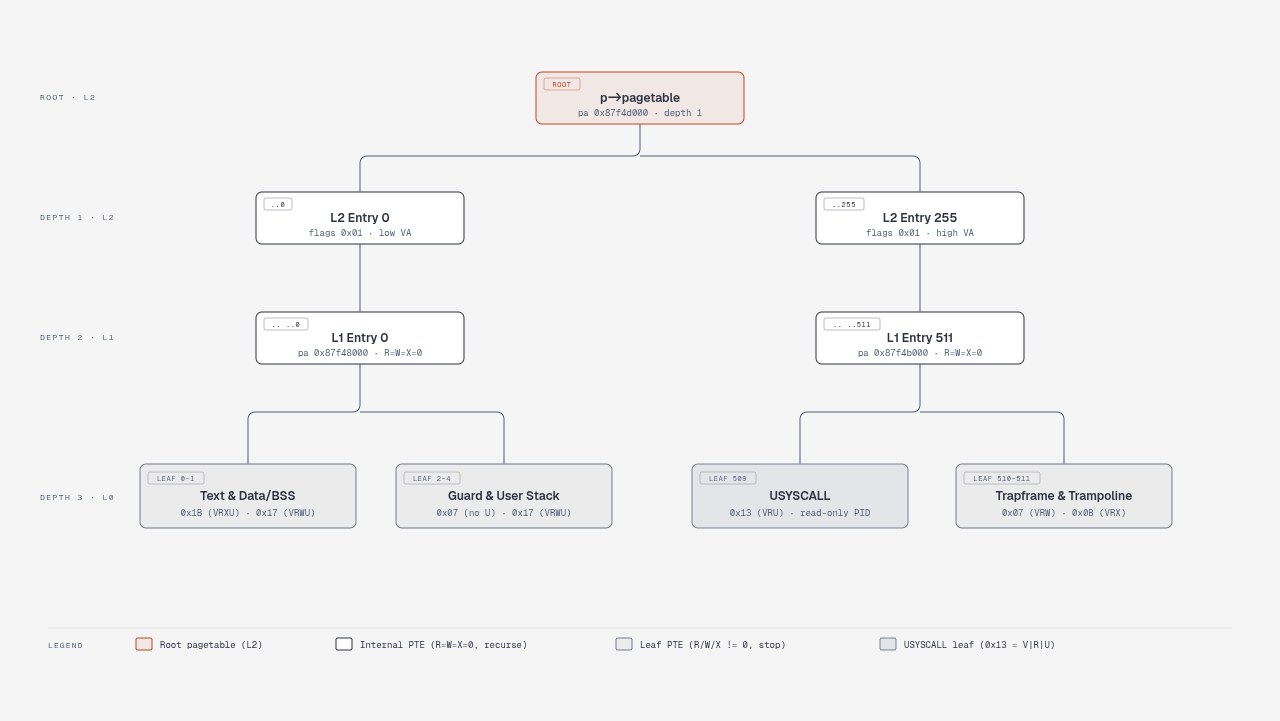
\includegraphics[width=0.96\textwidth]{images/vmprint_tree.png}
    \caption{Cấu trúc cây bảng trang Sv39 ba cấp của tiến trình
    \texttt{init} khi gọi \texttt{vmprint()}}
    \label{fig:vmprint_tree}
\end{figure}

\subsection{Kiểm thử và giải thích các trang lá}
Khi khởi động xv6 trên QEMU sau khi đã ghép đủ các phần của Lab 3 lên
nhánh \texttt{main}, kernel in ra cây bảng trang ba cấp của tiến trình
\code{init} rồi chạy vào shell bình thường:

\begin{lstlisting}[style=terminalstyle]
page table 0x0000000087f4d000
..0: pte 0x0000000021fd2401 pa 0x0000000087f49000
.. ..0: pte 0x0000000021fd2001 pa 0x0000000087f48000
.. .. ..0: pte 0x0000000021fd281b pa 0x0000000087f4a000
.. .. ..1: pte 0x0000000021fd1c17 pa 0x0000000087f47000
.. .. ..2: pte 0x0000000021fd1807 pa 0x0000000087f46000
.. .. ..3: pte 0x0000000021fd1417 pa 0x0000000087f45000
.. .. ..4: pte 0x0000000021fd1017 pa 0x0000000087f44000
..255: pte 0x0000000021fd3001 pa 0x0000000087f4c000
.. ..511: pte 0x0000000021fd2c01 pa 0x0000000087f4b000
.. .. ..509: pte 0x0000000021fd5413 pa 0x0000000087f55000
.. .. ..510: pte 0x0000000021fd5807 pa 0x0000000087f56000
.. .. ..511: pte 0x000000002000180b pa 0x0000000080006000
init: starting sh
$ echo vmprint-ok
vmprint-ok
\end{lstlisting}

Đối chiếu với Hình 3.4 trong sách xv6 \cite{xv6book} và yêu cầu đề bài
\cite{hcmus_os_lab3}, Bảng~\ref{tab:vmprint_leaves} giải thích những gì
từng trang lá chứa và ý nghĩa các bit quyền của chúng trong tiến trình
\code{init}.

\begin{table}[H]
    \centering
    \small
    \renewcommand{\arraystretch}{1.25}
    \begin{tabularx}{\textwidth}{l l l X}
        \toprule
        \textbf{Chỉ số L0} & \textbf{Cờ (Hex)} &
        \textbf{Bit quyền} &
        \textbf{Nội dung và quyền truy cập} \\
        \midrule
        \texttt{.. .. ..0} & \texttt{0x1B} & \code{V, R, X, U} &
        Trang chứa mã máy text và hằng số rodata của \texttt{init};
        user được đọc và thực thi nhưng không được ghi. \\
        \texttt{.. .. ..1} & \texttt{0x17} & \code{V, R, W, U} &
        Trang chứa dữ liệu data và BSS của \texttt{init}; user được
        đọc và ghi biến, tắt quyền thực thi. \\
        \texttt{.. .. ..2} & \texttt{0x07} & \code{V, R, W} &
        Trang guard page đặt ngay dưới stack; tắt \code{PTE\_U} để khi
        user tràn stack chạm vào thì bị trap báo lỗi trang. \\
        \texttt{.. .. ..3}--\texttt{4} & \texttt{0x17} &
        \code{V, R, W, U} &
        Hai trang user stack của \texttt{init} theo cấu hình
        \code{USERSTACK = 2} trong mã nguồn xv6-2024; user được đọc và
        ghi. \\
        \texttt{.. .. ..509} & \texttt{0x13} & \code{V, R, U} &
        Trang \texttt{USYSCALL} tại \code{TRAPFRAME - PGSIZE} chứa
        \code{struct usyscall}; user chỉ được đọc PID. \\
        \texttt{.. .. ..510} & \texttt{0x07} & \code{V, R, W} &
        Trang \texttt{TRAPFRAME} lưu $32$ thanh ghi của tiến trình khi
        có trap; tắt \code{PTE\_U} nên chỉ kernel truy cập được. \\
        \texttt{.. .. ..511} & \texttt{0x0B} & \code{V, R, X} &
        Trang \texttt{TRAMPOLINE} tại \code{MAXVA - PGSIZE} chứa mã
        trampoline; tắt \code{PTE\_U} và \code{PTE\_W} để user không
        đọc hay sửa được. \\
        \bottomrule
    \end{tabularx}
    \caption{Giải thích các trang lá và bit quyền của tiến trình
    \texttt{init}}
    \label{tab:vmprint_leaves}
\end{table}

Hình~\ref{fig:vmprint_result} là ảnh chụp màn hình QEMU lúc chạy thử
riêng phần \code{vmprint()} trên nhánh \texttt{feat/vmprint} trước khi
ghép thêm \code{USYSCALL} vào \texttt{main}, cho thấy shell vẫn nhận và
chạy lệnh \code{echo vmprint-ok} bình thường.

\begin{figure}[H]
    \centering
    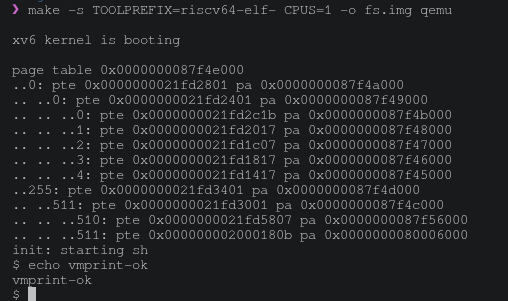
\includegraphics[width=0.82\textwidth]{images/vmprint-qemu.png}
    \caption{Kết quả chạy thử \texttt{vmprint()} trên QEMU tại nhánh
    \texttt{feat/vmprint}}
    \label{fig:vmprint_result}
\end{figure}
